\documentclass[10pt,twocolumn]{witseiepaper}
\setlength{\paperwidth}{210mm}
\setlength{\paperheight}{297mm}
\usepackage{KJN}
\usepackage{amsmath}
\usepackage{times}
\usepackage{flafter}
% Compatibility repair for the retained 2005 class with current LaTeX.
% The class expects a third caption argument; current hyperref supplies two.
\makeatletter
\long\def\@makecaption#1#2{%
  \vskip 5pt
  \setbox\@tempboxa\hbox{#1~:~#2}%
  \ifdim\wd\@tempboxa>\hsize
    {\noindent #1~:~#2\par}%
  \else
    \hbox to\hsize{\hfil\box\@tempboxa\hfil}%
  \fi
  \vskip 8pt}
\makeatother
\hypersetup{pdftitle={AI-Assisted E-Learning Recommendation Platform},pdfauthor={Gift Vundla},pdfsubject={Eligibility integration and reproducible verification}}



\begin{document}
\title{AI-Assisted E-Learning Recommendation Platform}
\author{Gift Vundla (2550723)}
\thanks{School of Electrical \& Information Engineering, University of the Witwatersrand, Johannesburg, South Africa\\Project 26P73.}
\abstract{Eligibility advice must distinguish unmet requirements from missing student facts and unverified rules. This investigation tested that distinction by connecting a source-linked rule engine to request interpretation and conversation state. Comparisons used 139 synthetic cases, a common 40-case baseline subset and 33 selected missing-fact cases. Adding School requirements raised code-based agreement from 119/139 (85.6\%) to 131/139 (94.2\%); rules-only reached 139/139 on structured inputs. No unsafe eligible answers occurred among 90 non-eligible references after the update. Clarification resolved 33/33 selected cases after one question and one scripted reply, compared with 13 correct decisions when omissions were treated as negative. Unrecognised history confirmations accounted for the eight remaining code-based failures. A separate diagnostic found an eligible decision with an outdated explanation. These findings identify evidence sufficiency, fact interpretation and explanation consistency as distinct checks on reliable advice. Cases and rules were development-informed, with shared source material and no recorded independent academic adjudication.}

\keywords{clarification, module eligibility, regression testing, rule integration}
\maketitle
\thispagestyle{empty}\pagestyle{empty}

\section{INTRODUCTION}
A module can match a student's interests without meeting registration requirements. Wits Electrical Engineering (EE, EFA03) and Information Engineering (IE, EFA04) impose programme restrictions, prerequisites and corequisites. Applicable conditions were assembled from Faculty rules \cite{wits}, course outlines and School guidance.

Academic advising systems support access to guidance \cite{empowered,khalil,tamas,nile,jiang}, while course recommenders address suitability \cite{chawana,islam,ibrahim}. The problem here was maintaining correct eligibility decisions when student histories were incomplete or ambiguously expressed. An omitted result cannot safely mean pass or fail; a missing institutional rule requires academic review rather than more student marks.

The investigation asked: \emph{How effectively did CurricuPath distinguish decidable eligibility cases from those needing student information or academic review, compared with rules-only and language-model baselines?} Integration and failure auditing compared conversational decisions with structured evaluation.

Three predictions guided the comparisons: complete inputs should preserve evaluator agreement (P1); clarification should outperform treating omissions as negative (P2); and School evidence should chiefly improve handbook-insufficient cases (P3). These predictions were development-informed, not preregistered. Evidence updates and clarification improved agreement; reply interpretation and inconsistent explanations remained failure points. The paper examines the design, comparisons and implications.

\section{LITERATURE REVIEW}
The relevant work addresses accessible advising, personalised recommendation, evidence sufficiency and the use of clarifying questions.

\begin{samepage}
Peer-advising, chatbots and AI agents address access to advice \cite{empowered,khalil,tamas,nile,jiang}. Kuhail et al.'s MyAdvisor used real advising scenarios and usability principles; students found it helpful and easy to learn \cite{khalil}. Usability, however, does not establish eligibility correctness. AdvisingWise retrieved institutional information, asked about academic backgrounds and required human-advisor validation before delivering responses \cite{jiang}. CurricuPath instead automated verified checks and referred insufficient evidence for review.
\end{samepage}

Chanaa and El Faddouli extracted concept prerequisites from linked data and matched them to course metadata \cite{chawana}; personalised and conversational recommenders also address course suitability \cite{islam,ibrahim}. Chanaa and El Faddouli reported normalised discounted cumulative gain at ten results (NDCG@10) of approximately 0.86 \cite{chawana}. This measures ranking relevance, not compliance with compulsory Wits registration conditions. CurricuPath therefore kept similarity-based discovery separate from source-linked eligibility checks. Ranking quality could not substitute for measuring correct, unsafe and unresolved decisions.

Joren et al. distinguish failure to use available information from insufficient retrieved context \cite{joren}. This motivated separating handbook-sufficient cases from those needing School evidence: a relevant description might still omit the applicable condition. The evidence comparison tested whether curriculum coverage explained failures that might otherwise be attributed to the model.

Aliannejadi et al. introduced Qulac to evaluate clarification through question selection and subsequent document retrieval \cite{qulac}. This motivates testing the outcome of clarification. CurricuPath's outcome was a registration decision: a reply could settle a compulsory prerequisite. Abstention research examines withholding unsupported answers \cite{abstention}. Here, the cause determined the next action: missing student facts prompted clarification; insufficient or disputed institutional evidence required academic review. The experiments therefore separated missing-fact handling from evidence completeness.

\section{DESIGN AND IMPLEMENTATION}
The backend combined the interpreted target, declared student facts and curriculum conditions, returning a decision, focused question or request for academic review.

\subsection{Representing curriculum requirements}
Modules, programme memberships, aliases, conditions and sources were stored separately. Rules retained their target, programme scope, condition and source locator, distinguishing compulsory combinations, such as Mathematics IA and IB, from accepted alternatives. Faculty rules \cite{wits} and School workbooks supported checking the encoded conditions. Module descriptions supported interest matching; the rule conditions determined eligibility.

Verified rules supported checks; disputed evidence, unavailable essential requirements and discretionary credit recognition required academic review. A language model could identify what the student meant, but could not supply a missing institutional rule. Programme, prerequisite, corequisite and exclusion checks applied recorded constraints, with repeat-module timetable checks as an additional gate. A completed prerequisite could not override a programme restriction or exclusion: eligibility required the combined conditions.

\subsection{Distinguishing unmet and unknown facts}
Student facts recorded completed, current, planned, not completed and unknown module states. A prerequisite required completed credit: current or planned study did not satisfy it. A corequisite could be completed, current or planned. Planned study therefore supported a conditional plan, not proof of enrolment.

The evaluator used three values: $T$ for satisfied, $F$ for unmet and $U$ for unknown. Equation (\ref{eq:logic}) combines compulsory conditions and accepted alternatives. Let $v(r)$ be the value of condition $r$. With ordering $F<U<T$,
\begin{equation}
 \begin{aligned}
 v\!\left(\bigwedge_i r_i\right)&=\min_i v(r_i),\\
 v\!\left(\bigvee_i r_i\right)&=\max_i v(r_i).
 \end{aligned}
\label{eq:logic}
\end{equation}
If one compulsory prerequisite was known to be unmet, learning another unknown result could not satisfy the whole requirement: $F\land U=F$. That question was unnecessary. A satisfied alternative, $T\lor U=T$, similarly removed the need to ask about another alternative. Source disputes were handled separately through review.

The engine retained an active unresolved condition, asked a decision-relevant question and re-evaluated the original target after the reply.

\subsection{Connecting requests, storage and evaluation}
FastAPI accepted typed target, programme and module-state fields \cite{fastapi}; React maintained interface state \cite{react}. The evaluator received these fields rather than answer prose. PostgreSQL held related catalogue records, SQLAlchemy represented their relationships, and Alembic managed schema changes \cite{alembic}. Source identity and verification status remained separate: an inspectable rule was not necessarily usable.

Catalogue replacement used a transaction \cite{sqlalchemy} so module, rule and source changes formed one update rather than exposing a partial import. Vectors were reused only when item identity, chunk kind and content hash matched, preventing reuse for changed text. BGE embeddings and pgvector supplied 384-dimensional similarity search \cite{pgvector,bge}. This supported discovery of related descriptions; recorded student facts and curriculum conditions still determined eligibility.

Controlled aliases and optional Gemini API interpretation produced a target, programme and declared statuses in structured fields \cite{gemini,structured}. Structured output constrained the format, not the truth of the interpretation. An uncertain target required resolution before evaluation. The session retained the target, pending requirement and known facts, allowing ``I have completed MATH1049A'' to update the original request. An unrecognised reply left the fact unknown, making reply interpretation a separately testable boundary.

Responses retained the target, outcome, rule checks and sources, locating identification failures separately from unresolved prerequisites. These traces and local tests supported implementation claims; documentation supported tool capabilities. Framework performance and embedding alternatives were not compared.

\subsection{Following one clarification through the system}
Mathematics II (MATH2014A) required Mathematics IA and IB, with listed old/current alternatives \cite[p.84]{wits}. In a separate local check of the corrected rule snapshot, the declared EFA03 profile had completed MATH1048A, left MATH1049A unknown and explicitly did not hold the older alternatives:

\noindent\emph{Student:} Can I take MATH2014A?\\
\emph{Advisor:} Have you completed MATH1049A?\\
\emph{Student:} I have completed MATH1049A.\\
\emph{Decision:} Eligible for the declared EFA03 profile.

The reply changed $T\land U=U$ to $T\land T=T$; failure would give $T\land F=F$. The answer supplied a fact without changing the rule.

The updated eligible decision retained a ``not satisfied'' requirements summary. Label-only checking would miss this contradiction. This diagnostic was separate from the archived benchmark.

\section{EXPERIMENTAL METHOD}
Experiments tested evidence effects, missing-fact clarification and divergence between conversational and structured evaluation.

\subsection{Cases and reference decisions}
The benchmark contained 139 synthetic cases: 49 eligible, 70 ineligible and 20 requiring manual review, across 70 EFA03 and 69 EFA04 profiles. Its recorded split was 36 development and 103 held-out cases. Code, name and informal wordings shared the same profile and reference. A frozen common subset contained 14 eligible, 20 ineligible and six manual-review cases. Twenty-one were labelled handbook-sufficient; 19 required further evidence or review.

Reference decisions were adopted from School workbooks supplied on 30 September 2026; cases recorded the target, profile, label and evidence rationale. For TS022 (ELEN3000A, EFA03), the record cited the EE Year 3 grid and Faculty rules \cite[p.81]{wits}: MATH3025A was a corequisite, absent from completed, current and planned study. Confirmation of complete current/planned lists supported ineligibility; otherwise omission required clarification. Section \ref{sec:failures} examines why the conversational path did not accept this confirmation.

No independent adjudicator was recorded. Shared source material meant agreement tested consistency, not independent academic correctness. Evidence sufficiency was a case annotation, not a guarantee that any retrieved page was adequate.

\subsection{System variants and evidence supplied}
Rules-only evaluated resolved targets and structured profiles. CurricuPath added interpretation and conversation state to that evaluator; no-clarification disabled questions. Handbook retrieval-augmented generation (RAG) generated decisions from passages. A structured-rules large language model (LLM) received encoded conditions and evidence states. The archived configuration recorded \texttt{gemini-3.5-flash-lite}, retrieval depth $k=20$ and one observation per case/wording.

The shared comparison retains original LLM observations and deterministic runs before and after adding School-grid requirements. Later grid-aware LLM reruns are outside this comparison. Thus the common 40 cases match the test population, but the post-grid deterministic and original LLM arms do not have identical evidence. Their difference cannot be attributed solely to model reasoning.

\subsection{Missing-fact experiment}
Clarification set v3 comprised 33 missing-fact cases, 33 matched known-fact controls and six irrelevant-unknown controls. Missing facts covered 12 single-prerequisite, six grouped-prerequisite, nine corequisite and six timetable-clash cases. Other clash partners were known. Cases selected for one-reply resolution favoured clarification. Developer-proposed labels awaited academic review.

CurricuPath asked and received a scripted reply; no-clarification could not ask; assume-absent treated omissions as negative; the oracle received structured resolving facts. No-clarification also failed to use a resolving fact supplied initially, so its unresolved outputs reflected an implementation limit. Assume-absent provided the substantive comparison with guessing. Recorded outcomes were correct, wrong or unresolved, with question counts. Reference agreement differed from independent correctness \cite{grras}.

\subsection{Scoring and implementation checks}
Macro-F1 gave equal weight to eligible, ineligible and manual-review decisions \cite{sokolova}. For each wording, it was computed as
\begin{equation}
 F_{\mathrm{macro}}=\frac{1}{3}\sum_{c=1}^{3}
 \frac{2TP_c}{2TP_c+FP_c+FN_c},
\label{eq:f1}
\end{equation}
where $TP_c$, $FP_c$ and $FN_c$ are true positives, false positives and false negatives for class $c$. Table \ref{tab:shared_safety} reports the mean of the three wording-specific scores. An unresolved output missed its reference class; it was not a correct manual-review decision. Unsafe rate counted eligible predictions on ineligible/manual-review references, divided by those references.

Clarification proportions used 95\% Wilson intervals. Wording variants repeated the same profiles, so pooled counts were descriptive rather than independent cases. Frozen hashes, raw outputs and scoring configurations were retained. Failure attribution used recorded statuses, targets and pending conditions.

Implementation checks were separate from the historical benchmark. Engine regressions covered programme restrictions, prerequisite states and clarification round trips. Repository tests were designed to compare PostgreSQL retrieval with the imported catalogue; these required an available database. Response checks used deliberately inconsistent fixtures. The focused run on 23 October 2026 made no hosted-model calls.

\section{RESULTS}
Added curriculum evidence improved agreement, and clarification resolved the selected missing-fact cases. The remaining failures identify where conversational inputs diverged from structured evaluation.

\subsection{Evidence and full-set agreement}
School evidence raised code-based agreement from 119/139 (85.6\%) to 131/139 (94.2\%) and reduced unsafe eligible decisions from 7/90 to 0/90. Post-update Macro-F1 was 0.9798, 0.9688 and 0.9716 for code, name and informal wording. Rules-only reached 139/139 on structured inputs. All remaining CurricuPath errors were unresolved outputs: withholding avoided unsafe eligibility, but still failed to provide the reference decision.

\subsection{Shared evidence and baseline results}
Both deterministic arms rose from 39/57 to 57/57 in the School-evidence group; handbook-sufficient outcomes were unchanged (Table \ref{tab:shared_evidence}; Figure \ref{fig:shared_evidence}). The frozen 40-case subset contributes 63 handbook-sufficient and 57 School-evidence-required observations across three wordings. Starred rows are deterministic updates made after inspecting earlier results.

\begin{table}[tb]
\caption{Correct decisions (\%) on the frozen 40-case subset.}
\label{tab:shared_evidence}
\centering
\small
\setlength{\tabcolsep}{3pt}
\begin{tabular}{p{29mm}rrr}
\hline
System & \shortstack{Handbook\\sufficient\\21/63} & \shortstack{School evidence\\required\\19/57} & \shortstack{All\\40/120}\\
\hline
Handbook RAG & 28.6\% & 31.6\% & 30.0\%\\
Structured-rules LLM & 38.1\% & 49.1\% & 43.3\%\\
Rules-only, before grid & 100.0\% & 68.4\% & 85.0\%\\
CurricuPath, before grid & 87.3\% & 68.4\% & 78.3\%\\
Rules-only, after grid* & 100.0\% & 100.0\% & 100.0\%\\
CurricuPath, after grid* & 87.3\% & 100.0\% & 93.3\%\\
\hline
\end{tabular}
\par\smallskip\noindent Headers show cases/inputs. *Development-informed results.
\end{table}

\begin{figure}[tb]
\centering
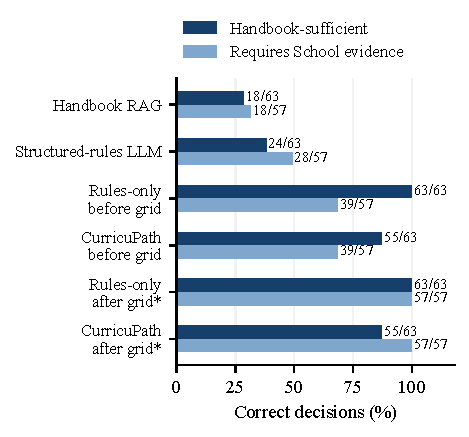
\includegraphics[width=\columnwidth]{shared_evidence.pdf}
\caption{Correct decisions by evidence sufficiency on the frozen subset, pooled across three wordings. Counts correspond to Table \ref{tab:shared_evidence}.}
\label{fig:shared_evidence}
\end{figure}

The evidence-specific improvement supports P3. Original RAG and structured LLM outcomes were lower, but different evidence representations and inputs prevented attributing that gap solely to reasoning.

\begin{table}[tb]
\caption{Classification performance and safety on the common 40-case subset.}
\label{tab:shared_safety}
\centering
\setlength{\tabcolsep}{3pt}
\begin{tabular}{lrr}
\hline
System & Mean Macro-F1 & Unsafe (\%)\\
\hline
CurricuPath* & 0.976 & 0.0\\
No clarification* & 0.976 & 0.0\\
Rules-only* & 1.000 & 0.0\\
Structured-rules LLM & 0.333 & 16.7\\
Handbook RAG & 0.278 & 38.5\\
\hline
\end{tabular}
\par\smallskip\noindent Mean Macro-F1 averages three wording-specific scores. Unsafe rate is the percentage of non-eligible inputs predicted eligible. *Grid-aware deterministic conditions.
\end{table}

Across the same 40 cases per wording, unsafe totals were 0/78 for each deterministic arm, 13/78 for structured LLM and 30/78 for RAG (Table \ref{tab:shared_safety}). Matching cases controlled the population, not the evidence supplied. CurricuPath and no clarification were identical here; their missing-fact behaviour required the separate P2 experiment.

\subsection{Why conversational requests remained unresolved}
\label{sec:failures}
History-completeness replies accounted for eight failures at every wording: TS022, TS041, TS077, TS078, TS081, TS089, TS110 and TS134. All had resolved targets and ineligible references. Despite the scripted reply, ``I have listed every module I am currently taking or planning'', clarification ended without an accepted status for MATH3025A, ELEN3012A or APPM3021A. The system continued asking about the module. Total unresolved decisions were 8, 12 and 11 for code, name and informal wording.

The rules-only adapter converted ``every module'' into a history-confirmed flag and treated omitted corequisites as absent. The conversational path failed to accept that confirmation, leaving them unknown. The difference therefore arose in transferring student information to the evaluator; these outputs did not demonstrate incorrect combination of rule conditions.

Module identification added four unresolved targets under name wording: TS027, TS057, TS064 and TS069. Informal wording failed on the same targets except TS057, whose Introduction to Machine Learning question included ELEN4025A and resolved. Responses requested a code or full name; the records did not establish a finer resolver cause. These cases motivate paired code/name checks.

\subsection{Clarification outcomes and interaction cost}
Clarification reached 33/33 correct decisions, matching the fully informed oracle; assume-absent reached 13/33 (Figure \ref{fig:clarification}). The latter produced 11 wrong and nine unresolved outputs, including three unsafe eligible answers among 16 ineligible references. No clarification left all 33 unresolved. For the selected scripted cases, the 95\% Wilson interval for 33/33 correctness was 89.57--100\%.

\begin{figure}[tb]
\centering
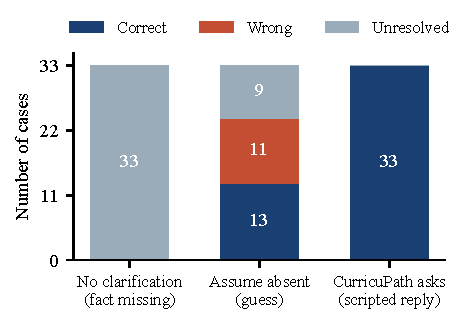
\includegraphics[width=\columnwidth]{shared_clarification.pdf}
\caption{Final decisions on 33 missing-fact cases after the allowed interaction. Labels were developer-proposed and replies scripted.}
\label{fig:clarification}
\end{figure}

Each missing-fact case required one question and one scripted reply, sometimes covering several statuses. CurricuPath asked no questions across the 39 known-fact or irrelevant-unknown controls, all of which ended correctly. The improvement supports P2 at this observed message cost; it does not establish student response time or abandonment.

\subsection{Focused implementation verification}
The focused run on 23 October passed 55 checks, skipped seven and recorded no failures. Checks covered unknown versus absent prerequisites, nested requirements, ambiguous module replies and clarification state. Response guards rejected constructed decision/text contradictions and unsupported module identifiers; schema checks exercised import mappings without a live database. The unavailable imported catalogue prevented all seven live PostgreSQL comparisons; the passing repository check exercised fallback construction. These selected checks left live-database equivalence unverified and did not re-estimate benchmark performance or cover every conversation.

\section{DISCUSSION}
The main result is that reliable eligibility advice depends on both the curriculum conditions and the way student facts reach them. A correct evaluator cannot compensate for a missing rule or a reply that has not been understood.

\subsection{What the predictions explain}
P1 was partly met. Rules-only reproduced structured references, while CurricuPath left some questions unresolved because it could not interpret history statements or identify module names. The eight shared failures show why the connection between conversation and evaluator matters. The Mathematics II diagnostic revealed another boundary: the decision had changed, but the explanation had not. Label accuracy alone did not detect this defect.

P2 was supported when the scripted reply supplied the missing status and the system accepted it. The history-statement failures show that asking a question is insufficient if its answer cannot be represented correctly. P3 was supported by improved agreement after adding School requirements, with the handbook-sufficient group unchanged. Together, these findings separate three causes of unreliable advice: insufficient institutional evidence, misunderstood student facts and inconsistent explanations.

\subsection{Design tradeoffs and limits of the evidence}
Requiring a resolved target prevented evaluation of an uncertain module, but made alias coverage important. TS057 succeeded when its code was present and failed on name-only wording. Preserving unknown statuses also avoided the assume-absent arm's three unsafe answers among 16 ineligible references, at the cost of leaving requests unresolved. The useful improvement is better interpretation while retaining the prerequisite checks.

Traceable rules made decisions inspectable, but created a continuing evidence-maintenance task. The School update followed inspection of earlier results, and the evaluator shared School material with the references. Some empty grid rows also relaxed design-module decisions; whether those rows meant no requirement rather than missing data still needed confirmation. Perfect rules-only agreement must be interpreted within those conditions. Declared review reasons tested routing, not autonomous discovery of institutional conflicts.

Synthetic profiles, reused templates, selected scripted replies, the small review group and single LLM observations limited generalisation despite the recorded held-out split. No independent academic adjudication or participant usability result was established. Historical post-grid results preceded later Faculty-rule corrections and the current grid-off runtime. Zero unsafe outputs on these references therefore did not establish a deployment risk bound.

\subsection{Practical improvements and further evaluation}
History completeness should be recorded separately for completed, current and planned modules: confirming one list must not imply credit in another. Verified title aliases should be extended, and explanations regenerated from the final evaluated state. Acceptance checks should pair code/name questions with the same profile and compare the decision, requirements summary and fact trace.

A stronger evaluation would freeze corrected rules and matched inputs, obtain independent academic decisions for fresh cases, test unseen replies and repeat model runs. A participant study would then measure time, abandonment and understanding, rather than treating message count as a complete measure of effort.

\newpage
\section{CONCLUSION}
CurricuPath's eligibility checks required sufficient institutional evidence and correctly interpreted student facts. After School updates, code-based questions matched 131/139 references (94.2\%); rules-only matched 139/139 structured cases. Clarification resolved 33/33 selected missing-fact cases after scripted replies, compared with 13 correct decisions when omissions were treated as negative.

Unrecognised history confirmations and an outdated explanation exposed failures beyond rule evaluation. Priority improvements are explicit history-completeness handling and explanations regenerated from final decisions. These synthetic cases used shared evidence for rules and references; independent academic adjudication and tests with unseen replies remain necessary before operational use.

\begin{thebibliography}{22}
\interlinepenalty=10000
\bibitem{wits} University of the Witwatersrand, Johannesburg, South Africa, \href{https://www.wits.ac.za/media/wits-university/students/academic-matters/documents/EBE_eBook.pdf}{\emph{2026 Senate Rules for the Faculty of Engineering and the Built Environment}}, 2026.
\bibitem{empowered} M.J.C. Samonte et al., ``\href{https://doi.org/10.1109/ICET67421.2025.11380449}{EmpowerED: A peer-to-peer learning and advising platform for college students in a Philippine university}'', in \emph{Proc. 5th International Conference on Educational Technology (ICET)}, IEEE, 2025.
\bibitem{khalil} M.A. Kuhail, H. Al Katheeri, J. Negreiros, A. Seffah and O. Alfandi, ``\href{https://doi.org/10.1080/10447318.2022.2074645}{Engaging students with a chatbot-based academic advising system}'', \emph{International Journal of Human--Computer Interaction}, vol.39, no.10, pp.2115--2141, 2023.
\bibitem{tamas} M. Tamascelli, O. Bunch, B. Fowler, M. Taeb and A. Cohen, ``\href{https://doi.org/10.1145/3696673.3723065}{Academic advising chatbot powered with AI agent}'', in \emph{Proc. ACMSE}, pp.195--202, ACM, 2025.
\bibitem{nile} M. Alaa et al., ``\href{https://doi.org/10.1109/NILES68063.2025.11232041}{NileAdvisor: AI-powered academic advising and recommendation system}'', in \emph{Proc. NILES}, IEEE, 2025.
\bibitem{jiang} W. Jiang, S. Wang, H. Eltigani, R. Haroon, A.B. Faisal and F. Dogar, ``\href{https://arxiv.org/abs/2511.05706}{AdvisingWise: Supporting academic advising in higher education settings through a human-in-the-loop multi-agent framework}'', arXiv:2511.05706, 2025.
\bibitem{chawana} A. Chanaa and N. El Faddouli, ``\href{https://doi.org/10.1186/s40561-024-00301-0}{Prerequisites-based course recommendation: Recommending learning objects using concept prerequisites and metadata matching}'', \emph{Smart Learning Environments}, vol.11, art.16, 2024.
\bibitem{islam} M.S. Islam and A.S.M.S. Hosen, ``\href{https://doi.org/10.3390/digital5020017}{Personalized course recommendation system: A multi-model machine learning framework for academic success}'', \emph{Digital}, vol.5, no.2, art.17, 2025.
\bibitem{ibrahim} Tan Chia Wei, M.H. Ahmad Hijazi, S. Alias, A.A.A. Ibrahim and M.F.I. Othman, ``\href{https://doi.org/10.18517/ijaseit.12.5.14798}{Intelligent course recommender chatbot using natural language processing}'', \emph{International Journal on Advanced Science, Engineering and Information Technology}, vol.12, no.5, pp.1915--1920, 2022.
\bibitem{joren} H. Joren, J. Zhang, C.-S. Ferng, D.-C. Juan, A. Taly and C. Rashtchian, ``\href{https://proceedings.iclr.cc/paper_files/paper/2025/file/33dffa2e3d2ab74a783d1a8c292f66d9-Paper-Conference.pdf}{Sufficient context: A new lens on retrieval augmented generation systems}'', in \emph{Proc. ICLR}, 2025.
\bibitem{qulac} M. Aliannejadi, H. Zamani, F. Crestani and W.B. Croft, ``\href{https://doi.org/10.1145/3331184.3331265}{Asking clarifying questions in open-domain information-seeking conversations}'', in \emph{Proc. SIGIR}, pp.475--484, ACM, 2019.
\bibitem{abstention} B. Wen, J. Yao, S. Feng, C. Xu, Y. Tsvetkov, B. Howe and L.L. Wang, ``\href{https://aclanthology.org/2025.tacl-1.26/}{Know your limits: A survey of abstention in large language models}'', \emph{Transactions of the Association for Computational Linguistics}, vol.13, pp.529--556, 2025.
\bibitem{fastapi} FastAPI, ``Request body.'' \url{https://fastapi.tiangolo.com/tutorial/body/}, 2026. Accessed: 22 Oct.2026.
\bibitem{react} React, ``Managing state.'' \url{https://react.dev/learn/managing-state}, 2026. Accessed: 5 Oct.2026.
\bibitem{alembic} Alembic, ``Tutorial: creating a migration script.'' \url{https://alembic.sqlalchemy.org/en/latest/tutorial.html\#create-a-migration-script}, 2026. Accessed: 22 Oct.2026.
\bibitem{sqlalchemy} SQLAlchemy, ``Working with transactions and the DBAPI.'' \url{https://docs.sqlalchemy.org/en/20/tutorial/dbapi_transactions.html}, 2026. Accessed: 22 Oct.2026.
\bibitem{pgvector} pgvector, ``Vector type and similarity search.'' \url{https://github.com/pgvector/pgvector\#vector-type}, 2026. Accessed: 5 Oct.2026.
\bibitem{bge} Beijing Academy of Artificial Intelligence, ``BAAI/bge-small-en-v1.5: model card.'' Hugging Face model hub. \url{https://huggingface.co/BAAI/bge-small-en-v1.5}, 2026. Accessed: 20 Oct.2026.
\bibitem{gemini} Google AI for Developers, ``Gemini 3.5 Flash-Lite.'' \url{https://ai.google.dev/gemini-api/docs/models/gemini-3.5-flash-lite}, 2026. Accessed: 3 Oct.2026.
\bibitem{structured} Google AI for Developers, ``Structured outputs: Gemini API.'' \url{https://ai.google.dev/gemini-api/docs/structured-output}, 2026. Accessed: 5 Oct.2026.
\bibitem{grras} J. Kottner, L. Audig\'e, S. Brorson, A. Donner, B.J. Gajewski, A. Hr\'objartsson, C. Roberts, M. Shoukri and D.L. Streiner, ``\href{https://doi.org/10.1016/j.jclinepi.2010.03.002}{Guidelines for reporting reliability and agreement studies (GRRAS) were proposed}'', \emph{Journal of Clinical Epidemiology}, vol.64, no.1, pp.96--106, 2011.
\bibitem{sokolova} M. Sokolova and G. Lapalme, ``\href{https://doi.org/10.1016/j.ipm.2009.03.002}{A systematic analysis of performance measures for classification tasks}'', \emph{Information Processing \& Management}, vol.45, no.4, pp.427--437, 2009.
\end{thebibliography}
\end{document}
